\chapter{Base maps}

\pagestyle{fancy}
\fancyhf{}
\fancyhead[OC]{\leftmark}
\fancyhead[EC]{\rightmark}
%\renewcommand{\footrulewidth}{1pt}
\cfoot{\thepage}

%%%%%%%%%%%%%%%%%%%%%%%%%%%%%%%%%%%%%%%%%%%%%%%%%%%%%%%%%%%
%%%%%%%%%%%%%%%%%%%%%%%%%%%%%%%%%%%%%%%%%%%%%%%%%%%%%%%%%%%

A base map provides a background to give context to your map.\\

Always make sure you base map remains your bottom most layer within the \textit{Layers Panel} - this will become more clear later.\\

You may wish to make any data layers that we put on top of a base map slightly transparent so that you can see some of the detail of the base map - a styling preference, so your choice.\\

I will introduce you to two options of a base map. There are many more.\\

\section{Add a simple world map}

In the coordinate field (in the status bar) type \textit{world} \& press enter to get a quick map of the world on the canvas.\\

Visual representation of a World map (countries) will appear in the map canvas.\\
The layer name will appear in the \textit{Layers Panel}\\
Notice the projection = EPSG4326.\\
Now the Layers Styling panel (if open) will have content.\\

\begin{figure}[!h]
	\centering
	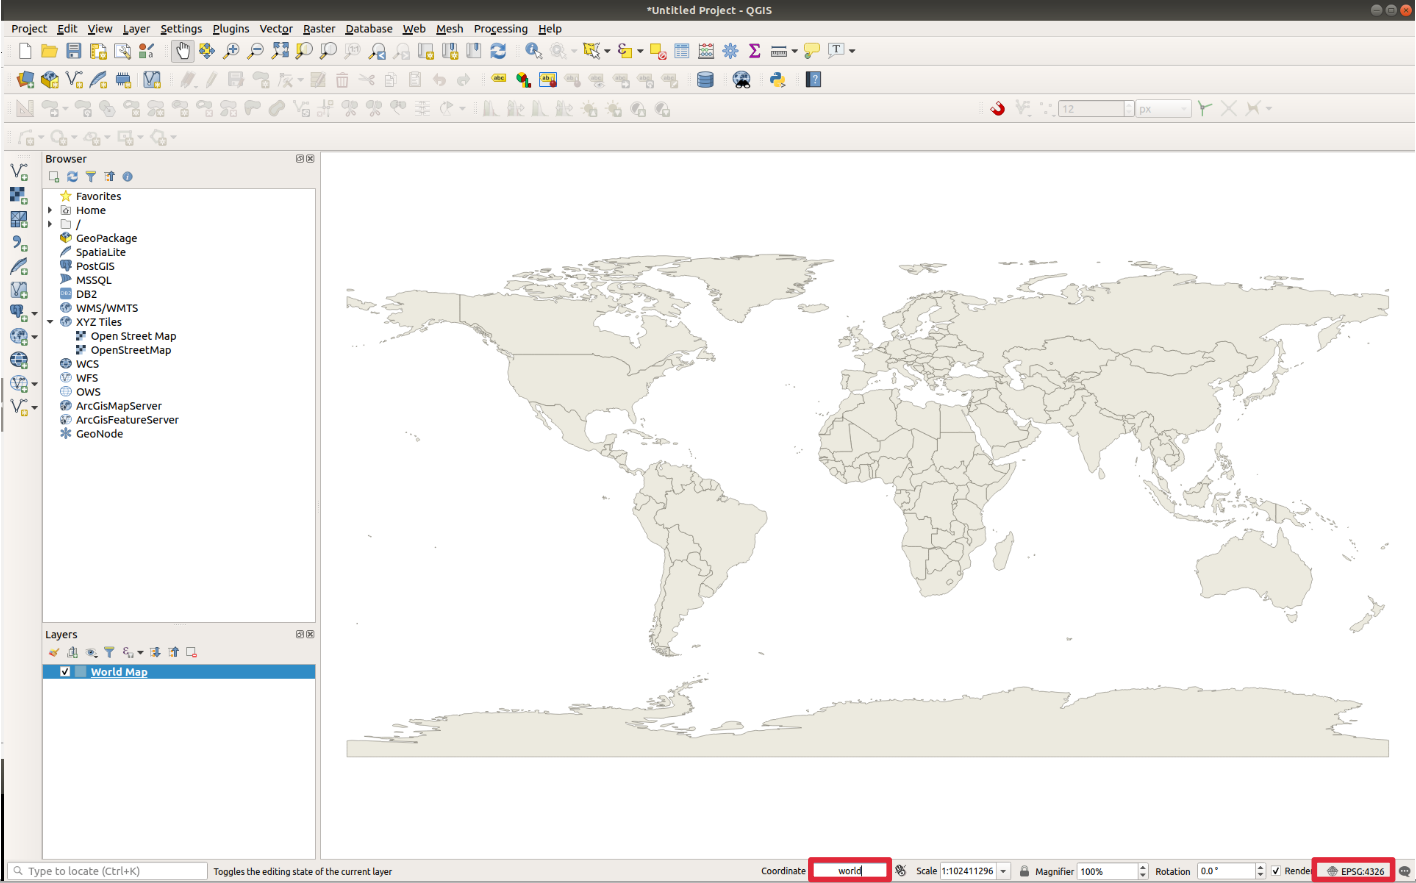
\includegraphics[width=0.7\textwidth]{images/coordinate_field_world.png}
	\caption{World map (type "World" in the co-ordinate field in the status bar)}
	\label{ft_fig_firstfig3}
\end{figure}

%world_map_EPSG4326_incl_Layer_Styling.png

\section{Add open street map}

This option requires internet connection (it is a predefined online datasource).\\

In Browser Panel find \textit{XYZ Tiles} $\rightarrow$ \textit{OpenStreetMap} and add it to your map canvas by either:
\begin{enumerate}
	\item double clicking
	\item drag and drop it outside of the Browser panel
\end{enumerate}

It will now appear in the \textit{Layers Panel}.\\
%Notice the projection = EPSG3857.\\
%Within the \textit{Layers Panel}, press and hold the layer name OpenStreetMap and drag it to become the bottom layer.\\

%\begin{figure}[!h]
%	\centering
%	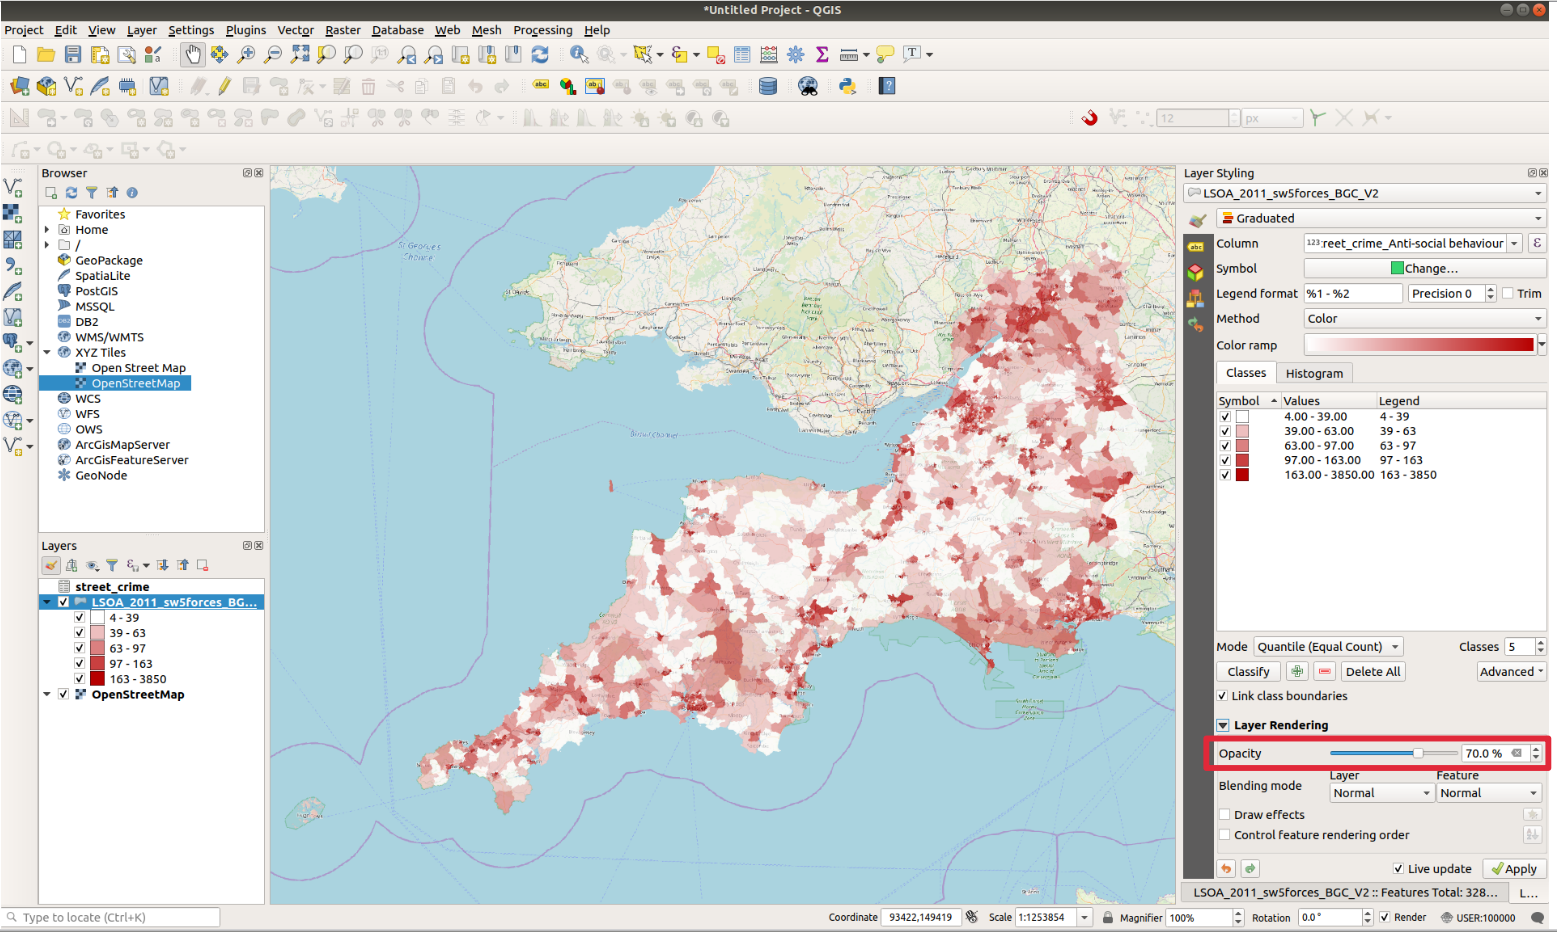
\includegraphics[width=1\textwidth]{images/add_base_map.png}
%	\caption{}
%	\label{ft_fig_firstfig3}
%\end{figure}
\begin{figure}[!h]
	\centering
	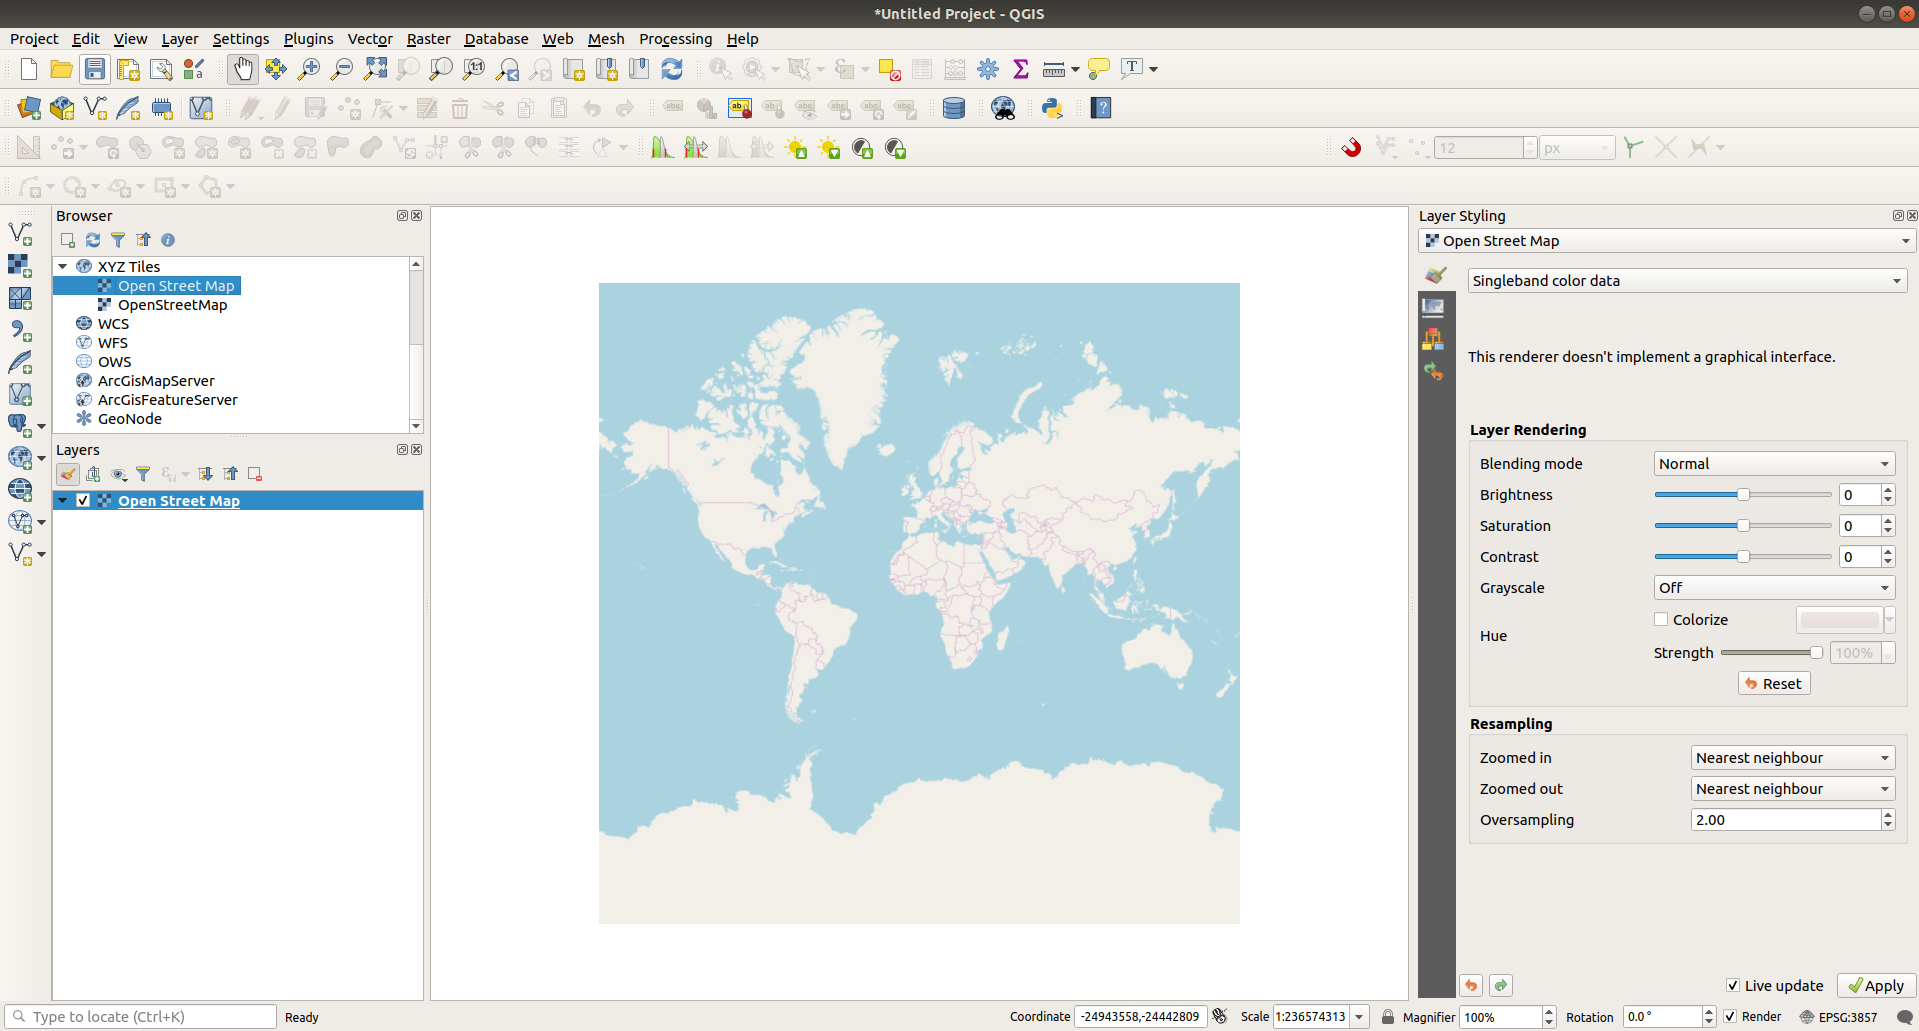
\includegraphics[width=1\textwidth]{images/openstreetmap_EPSG3857.png}
	\caption{Open Street Map to use as a base map}
	\label{ft_fig_firstfig3}
\end{figure}

%openstreetmap_EPSG4326.png

If you do use OpenStreetMap, please pay attention to their copyright and licence
\url{https://www.openstreetmap.org/copyright}. We will accredit this data in our \textit{print layout} that we create at the end of the tutorial.